\subsubsection{Customer Facebook Login}
			To accompany this diagram, read the Scenario \hyperref[sec:CustomerFacebookLoginScenario]{S.5}.

				\begin{table}[htpb]
					\centering
					\label{tab:CustomerFacebookLoginDiagramTable}
					\begin{tabularx}{\textwidth}{lp{9cm}}
						\hline
						\hline
							\textbf{Subject}
						& 
							\textbf{Description}\\
						\hline
							Actors	       &  Customer, myTaxiService Mobile Application, myTaxiServiceServer, Facebook System.\\
						\hline
							Preconditions  &  Registered User must have a Facebook account registered in the myTaxiService System.\\
						\hline
							Execution      &  1.~Customer opens the myTaxiService Mobile Application.\\
							               &  2.~myTaxiService Mobile Application shows the Login screen.\\
							               &  3.~Customer clicks on the "Login with Facebook" button.\\
							               &  4.~myTaxiService facebook login function is called and the homepage is showed to the Customer if the Facebook login is successful.\\
						\hline
							Postconditions &  Customer is logged in.\\
						\hline
							Exceptions     &  1.~The Customer disconnects before the homepage is showed.\\
									
						\hline
						\hline
					\end{tabularx}
				\end{table}
				
				%sto
				\begin{figure}[H]
					\centering
					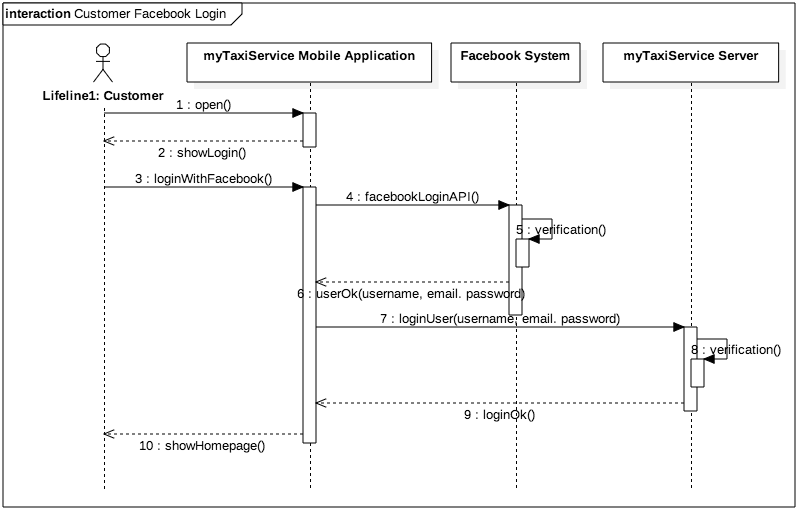
\includegraphics[width=\textwidth, scale=0.5]{IMG/InteractionDiagrams/CustomerFacebookLogin.png}
					\caption{FacebookLogin Interaction Diagram}\label{sec:FigureCustomerFacebookLogin}
				\end{figure}